\chapter{Die Messung als Zufallsprozess}
\label{chap:fehler}

\section{Modell und Experiment}
\label{chap:fehler:sec:modell}

In der Physik ist es oft weder möglich noch notwendig, die gesamte Komplexität eines Sachverhalts zu erfassen. Man verwendet daher Modelle: vereinfachte, mathematische Beschreibungen, die eine ausreichende Grundlage bieten, um  Vorhersagen über das Verhalten eines bestimmten Systems treffen zu können. Ein besonders wichtiges Beispiel für ein physikalisches Modell ist der sogenannte getriebene und gedämpfte harmonische Oszillator. Mit diesem Modell kann man zahlreiche Phänomene näherungsweise beschreiben, zum Beispiel die Bewegung des Planeten um einen Stern, die Bewegung einer Schaukel oder den Strom in einem RLC-Stromkreis. Mathematisch kann der Oszillator beschrieben  werden als 
\begin{align}
\ddot{x} + \Gamma \dot{x} + \omega_0^2 x = \frac{F ( t )}{m}\,.
\end{align}
Hierbei ist $x$ die Auslenkung, \gls{gl:Gamma} die Abklingkonstante, \gls{gl:omega_0} die Resonanzfrequenz multipliziert mit $2\pi$ (die sogenannte Kreisfrequenz), \gls{gl:F} die Kraft, \gls{gl:t} die Zeit und \gls{gl:m} die Masse. Wenn die Kraft durch eine cosinusförmige Oszillation mit konstanter Amplitude und Phase gegeben ist,
\begin{align}
F(t) = F_0 \cos(\omega t)\,.
\end{align}
können wir für jede Treibfrequenz $\omega$ eine zeitunabhängige Lösung erhalten:
\begin{align}
x(\omega) = \frac{F(\omega)/m}{\omega_0^2-\omega^2+i\omega\Gamma}\,.
\end{align}
Daraus lassen sich schliesslich die Amplitude $x_0(\omega) = \lvert x \rvert$ und die Phase $\phi(\omega) = \frac{\mathrm{Im}[x]}{\mathrm{Re}[x]}$ des Systems berechnen. \\

Um die Korrektheit eines Modells zu überprüfen, wird ein Experiment benötigt. Als einfaches Beispiel betrachten wir hier einen mit einem Quartzkristall gefüllten Kondensator. Ein Quartzkristall ist ein sogenanntes Piezomaterial, in dem das Anlegen einer elektrischen Spannung $U_{\mathrm{out}}$ eine mechanische Spannung erzeugt. Eine periodische Spannung nahe der mechanischen Resonanzfrequenz des Quartzkristalles führt deshalb zu einer Schwingung. Diese Schwingung ihrerseits induziert wiederum eine Spannung $U_{\mathrm{in}}$ im Kondensator, die wir messen können. Dieses System wollen wir als einen getriebenen und gedämpften harmonischen Oszillator mit $U_{\mathrm{in}} = x$ modellieren. \\

Um unser Modell zu verifizieren, führen wir ein einfaches Experiment durch, bei dem wir die Treibfrequenz einer angelegten Spannung über die Resonanzfrequenz des Quartzkristalls streichen und die Amplitude und Phase von $U_{\mathrm{in}}$ aufzeichnen. Ein Vergleich der theoretisch erwarteten und gemessen Kurven zeigt auf, dass wir das erwartete Verhalten des Oszillators nicht vollständig reproduzieren können (siehe Figur \ref{fig:oszillator}). Der Grund hierfür ist, dass  das aufgezeichnete Signal zusätzlich zu der durch die Schwingung des Kristalls induzierten Spannung auch eine zweite Spannungskomponente enthält. Die zweite Komponente entsteht durch die direkte kapazitive Kopplung zwischen den Kondensatorplatten und ist unabhängig von der Quartzschwingung. Dieses zusätzliche Signal können wir korrekt modellieren, indem wir unser Modell durch eine komplexe, konstante Zahl $C$ erweitern. Häufig realisieren wir durch ein Experiment also, dass wir unser Modell anpassen müssen, um das Verhalten eines Systems adäquat beschreiben zu können.  

\begin{figure}[H]
\centering
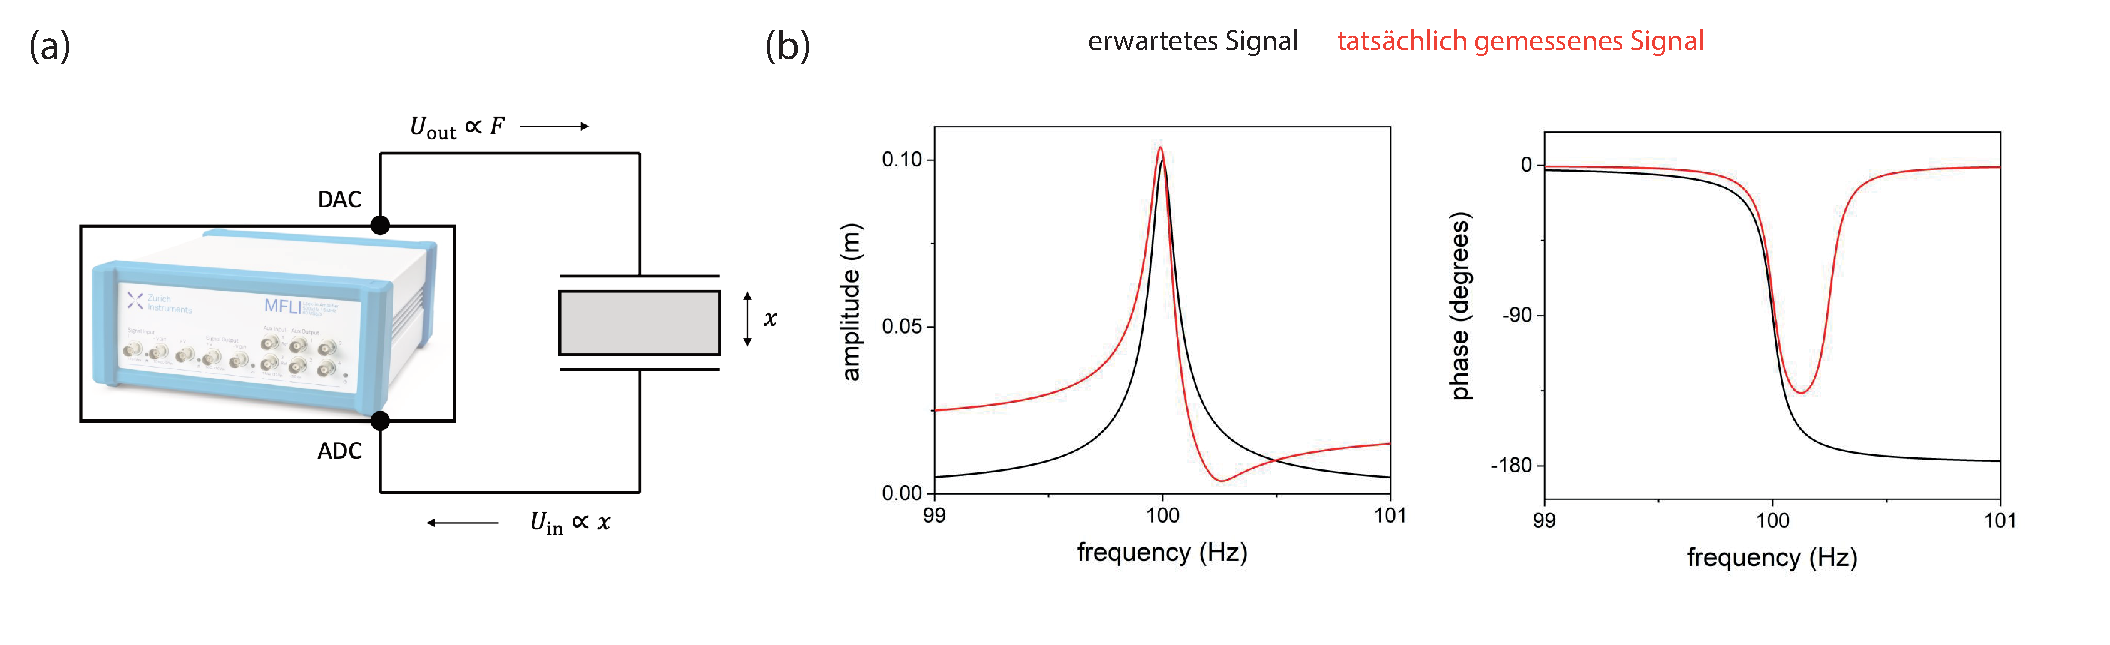
\includegraphics[width=0.9\textwidth]{Figures/modellundexperiment.pdf}
\caption{(a): Schematische Visualisierung des Versuchsaufbaus. (b): Erwartetes (schwarz) und tatsächlich gemessenes Signal (rot) für Amplitude (links) und Phase (rechts) von U$_{\mathrm{in}}$. }
\label{fig:oszillator}
\end{figure}

 Ein Modell kann allerdings niemals bewiesen, sondern immer nur widerlegt werden. Soll heissen: Auch wenn unser Experiment keine Lücken im Modell aufdeckt, könnte es immer noch ein anderes, alternatives Modell geben, das die gleiche Beobachtung erklären würde. Deckt unser Experiment hingegen eine Lücke auf, ist das Modell widerlegt worden und muss verworfen, beziehungsweise angepasst werden. Ein wichtiger Bestandteil dieses Prozesses, des Überprüfens eines Modells anhand eines Experiments, ist selbstverständlich die Analyse der gemessenen Daten. Kein Experiment ist komplett fehlerfrei, doch idealerweise sollten wir zwischen Fehlern des Modells und Fehlern des Experiments unterscheiden können. In diesem Kapitel wollen wir uns daher im Detail mit Messfehlern beschäftigen. 

\section{Messfehler}
\label{chap:fehler:sec:messfehler}

\begin{center}
\begin{tcolorbox}[enhanced,width=6in,center upper,
    fontupper=\large,drop fuzzy shadow southwest,
    colframe=blue!50!black,colback=blue!10]
Für dieses Unterkapitel ist ein Jupyter-Notebook verfügbar. Siehe \gitresource{Messfehler.ipynb}  
\end{tcolorbox}
\end{center}

\subsection{Was ist ein Messfehler?} % oder : Definition? 

Um zu verdeutlichen, was ein Messfehler ist, wollen wir zunächst ein einfaches Beispiel betrachten. Wir messen mit dem Beschleunigungssensor eines Smartphones die Erdbeschleunigung  \gls{gl:g}.\footnote{Dafür kann zum Beispiel die App Phyphox verwendet werden, Download möglich auf \href{https://phyphox.org}{phyphox.org}} Da der Wert der Erdbeschleunigung bereits mit sehr hoher Genauigkeit gemessen wurde,  erwarten wir schon vor der Messung ein bestimmtes Messergebnis, \gls{gl:xtilde}. Dieser erwartete Wert \gls{gl:xtilde} ist eine Abschätzung des tatsächlichen Werts von $g$, den wir (grundsätzlich) nicht kennen.  Während unserer ersten Messung von \gls{gl:g} erhalten wir nun einen Wert $x_1 \neq \Tilde{x}$. Der Abstand zwischen $x_1$ und \gls{gl:xtilde} ist der Fehler $e$ unserer Messung:
\begin{align}
\gls{gl:e} = \Tilde{x} - x_1\,.
\label{eq:messfehler}
\end{align}
Ein solcher Messfehler kann verschiedene Ursachen haben. Entweder kann bei der Messung selbst ein Fehler auftreten, z.B. durch  Ableseungenauigkeit, der Messung des falschen Parameters oder der ungenügenden Kalibration eines Messgerätes. Oder aber die Messung wird beeinflusst von (unbekannten) äusseren Faktoren wie z.B. Temperatur oder Luftfeuchtigkeit. \\

In jedem Fall gibt es bei einem Messvorgang für die gemessene Grösse einen tatsächlichen Wert, der - wie oben bereits erwähnt -  grundsätzlich unbekannt ist. Der erwartete Wert \gls{gl:xtilde} kann wie z.B. hier ein Literaturwert sein, oder ein theoretisch vorhergesagter Wert. Manchmal haben wir jedoch keine genaue Erwartung an den zu messenden Wert und können somit auch nicht direkt erkennen, ob unsere Messung stark vom erwarteten Wert abweicht. Somit müssen wir eine Möglichkeit finden, die Genauigkeit unserer Messung abzuschätzen und den Messfehler experimentell zu charakterisieren. 

%Alte Formulierung Laura: 
%Selbstverständlich kennen wir normalerweise den Erwartungswert \gls{gl:xtilde} der zu messenden Grösse nicht und können somit auch nicht den Fehler unserer Messung genau beziffern.\footnote{Ausnahmen sind Messungen von Naturkonstanten (z.B. \gls{gl:c}) oder anderen häufig verwendeten Werten (z.B. \gls{gl:g}), für die vertrauenswürdige Literaturwerte durch früheren Messungen vorliegen.}  Somit müssen wir eine Möglichkeit finden, die Genauigkeit unserer Messung abzuschätzen und den Messfehler experimentell zu charakterisieren. 

% Martin:
%Der erwartete Wert kann wie z.B. hier ein Literaturwert sein, oder ein theoretisch vorhergesagter Wert. Manchmal haben wir aber auch keine genaue Erwartung an den zu messenden Wert.
%In jedem Fall gibt es jedoch einen tatsächlichen Wert, der grundsätzlich unbekannt ist. 


\subsection{Systematische und zufällige Fehler}

Im Folgenden wollen wir zwischen systematischen und zufälligen Messfehlern unterscheiden.  Systematische Abweichungen sind konstante oder sich auf der Zeitskala unseres Experimentes nur sehr langsam ändernde Abweichungen des gemessenen Wertes vom tatsächlichen Wert. Solche systematischen Fehler können z.B. durch die falsche Kalibration einer Messapparatur zustande kommen. Sie können manchmal mittels einer Kontrollmessung einer bekannten Grösse in derselben Messapparatur aufgedeckt und eliminiert werden. Zufällige Fehler hingegen sind schnell fluktuierende Abweichungen, die bei jeder Durchführung des Experiments variieren und in der Regel nicht durch frühere Beobachtungen vorhergesagt werden können. Im Gegensatz zu systematischen Messfehlern sind zufällige Messfehler deutlich schwieriger auszuschliessen. Sie können lediglich reduziert, aber nicht vollständig eliminiert werden. Eine Messung, die zu Daten führt, die keine zufälligen Fehler zeigen, sollte misstrauisch machen.

\subsection{Statistische Analyse durch wiederholtes Messen} 

Der Messfehler lässt sich durch wiederholtes Messen $x_1$, $x_2$, $x_3$, ..., $x_N$  unserer Messgrösse statistisch analysieren. Aus unseren Messergebnissen, unserer sogenannten Stichprobe, können wir einen  \textbf{empirischen Mittelwert}
\begin{align}
\gls{gl:xoverline} = \frac{1}{N} \sum^N_{n = 1} x_n
\label{eq:empmean}
\end{align}
und eine \textbf{empirische Varianz}
\begin{align}
\gls{gl:deltax2}  = \frac{1}{N-1} \sum^N_{n = 1} \left( x_n - \gls{gl:xoverline} \right) ^2
\label{eq:empvar}
\end{align}
berechnen. Häufig wird auch die empirische Standardabweichung \gls{gl:deltax}, die Quadratwurzel der empirischen Varianz, verwendet. Sie ist somit ein Mass für systematische Fehler. Die \textbf{Präzision} einer Messung beschreibt die zufällige Verteilung der Messwerte um deren Mittelwert und ist somit ein Mass für zufällige Fehler. Beide Fehler lassen sich anschaulich in einem \textbf{Histogramm} darstellen, indem wir den Messbereich in gleich grosse ``Bins'' diskretisieren und die Messergebnisse innerhalb jedes Bins zählen (siehe Fig.~\ref{fig:messfehler1}).   \\

Kehren wir nun zu unserem anfänglichen Beispiel zurück. Wir führen $N$ Messungen von \gls{gl:g} durch und speichern die Ergebnisse in einem Numpy-Array $g$ ab. Ebenfalls speichern wir die zugehörigen Zeitpunkte $t$ der Messungen. In einem ersten Schritt visualisieren wir diese Daten in einem sehr einfachen Plot
\begin{lstlisting}[language = Python]
plt.plot(t, g)
\end{lstlisting}
und bestimmen den empirischen Mittelwert und die empirische Varianz der Stichprobe. Dies kann sowohl mithilfe der in \ref{eq:empmean} und \ref{eq:empvar} angegebenen Formeln   
\begin{lstlisting}[language = Python]
mean = np.sum(g)/N
var = np.sum((g-mean)**2)/(N-1)
\end{lstlisting}
oder aber durch Verwendung der Funktionen der numpy-Bibliothek. 
\begin{lstlisting}[language = Python]
mean = np.mean(g)
var = np.var(g)
\end{lstlisting}
geschehen. Hierbei ist zu beachten, dass die so berechnete Varianz nicht die empirische Varianz ist. Um die empirische Varianz zu erhalten muss die Varianz mit einem Faktor $\frac{N}{N-1}$ multipliziert werden.\\

Wir generieren nun unsere ``Bins'', um den Messbereich zu diskretisieren, und zählen die Messergebnisse pro Bin. Zur Auswahl der Breite der Bins ist die anfängliche Visualisierung der Daten hilfreich. Da die vertikale Auflösung unserer Messung ohnehin durch die Präzision unseres Messgerätes limitiert ist, wählen wir relativ breite Bins.  
\begin{lstlisting}[language = Python]
n_bins = 14+1 # Anzahl an Bins
bin_size = 0.005 # Breite des Bins 
bins = np.linspace(9.76, 9.76+bin_size*(n_bins-1), n_bins) 
# Initialisiere Numpy Array um Anzahl Messergebnisse pro Bin
# zu speichern
occurrence = np.zeros(n_bins)
offset = np.min(bins)//bin_size + 1
# Iteriere ueber alle Datenpunkte
# Bestimmte den Index des Bins, in den sie fallen
# Inkrementiere die Anzahl Ereignisse in diesem Bin um 1
for gx_i in gz:
    index = int(gx_i//bin_size-offset)
    occurrence[index] = occurrence[index] + 1
\end{lstlisting}
Nun können wir sehr einfach das Histogramm erstellen und den empirischen Mittelwert, die empirische Standardabweichung sowie den erwarteten Wert einzeichnen. Hierbei normalisieren wir unser Histogramm bereits entsprechend, um eine prozentuelle Wahrscheinlichkeit zu erhalten.\footnote{``Normalisieren'' bezeichnet die Multiplikation mit einem Faktor (in diesem Fall $A$), um der berechneten Grösse eine konkrete Bedeutung zuweisen zu können. In unserem Fall soll die Normierung erreichen, dass die Summe der Histogrammwerte 1 (oder 100 Prozent) ergibt.} 
\begin{lstlisting}[language = Python]
A =  N
g_theo = 9.78 
plt.bar(bins, occurrence/A, width = bin_size)
plt.vlines(g_theo, 0, np.max(occurrence)/A)
plt.vlines(mean, 0, np.max(occurrence)/A)
plt.vlines(mean + np.sqrt(var), 0, np.max(occurrence)/A)
plt.vlines(mean - np.sqrt(var), 0, np.max(occurrence)/A )
\end{lstlisting}
 Der von uns bestimmte Mittelwert weicht vom erwarteten Wert von  \gls{gl:g} ab, unsere Messung ist also nicht genau,  allerdings liegt der erwartete Wert noch innerhalb der empirischen Standardabweichung der Messung.
 % Hier fehlt noch ein abrundender Absatz

\begin{figure}[H]
\centering
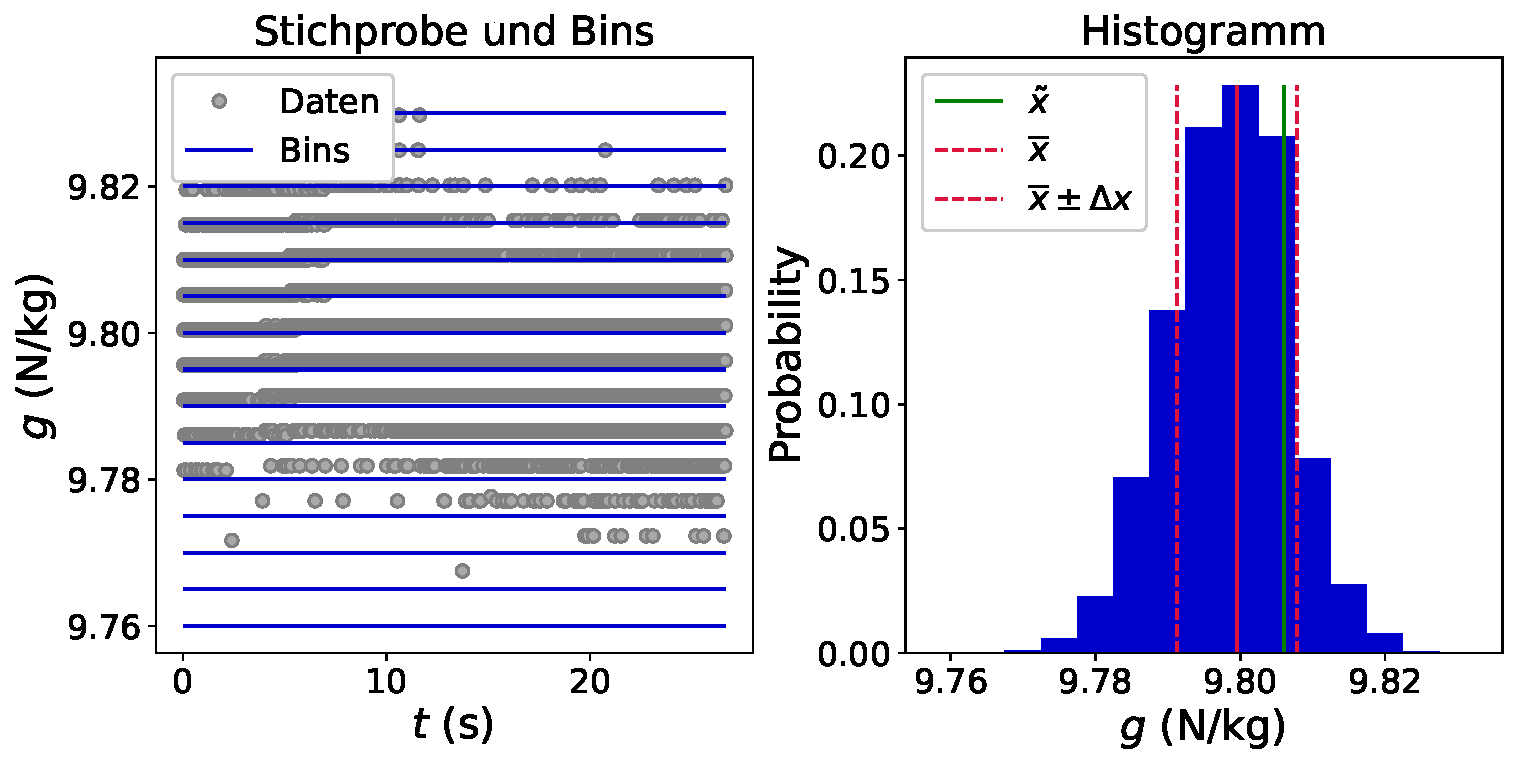
\includegraphics[width=0.9\textwidth]{Figures/messfehler1.pdf}
\caption{Statistische Analyse einer Messung von \gls{gl:g}. \textbf{Links:} Gemessene Datenpunkte (graue Punkte) als Funktion der Zeit $t$. Die Kanten der ``Bins'' sind als horizontale Linien indiziert. Aufgrund der limitierten vertikalen Auflösung der Messung arbeiten wir mit einer relativ geringen Anzahl von Bins.  \textbf{Rechts:} Das resultierende Histogramm der Stichprobe. Die Anzahl der Messergebniss pro Bin wurden für diese Darstellung bereits der Anzahl der Datenpunkte $N$ normalisiert, sodass die Summe aller Histogrammwerte 1 ergibt. Der erwartete Wert \gls{gl:xtilde} für die Erdbeschleunigung, sowie empirischer Mittelwert und empirische Standardabweichung sind eingezeichnet. }
\label{fig:messfehler1}
\end{figure}
%  Die Anzahl der Messergebniss pro Bins wurden für diese Darstellung bereits mit dem Produkt aus Anzahl der Datenpunkte $n$ und Bin-Breite normalisiert.

\section{Wahrscheinlichkeitsverteilungen}
\label{chap:fehler:sec:frequentistisch}

Im bisherigen Verlauf dieses Kapitels haben wir gelernt, wie wir zufällige Messfehler anhand der wiederholten Durchführung einer Messung charakterisieren können. Ein wichtiges Resultat dieser Analyse war hierbei das diskrete Histogramm der Ereignishäufigkeiten (siehe Fig.~\ref{fig:messfehler1}), die wir intuitiv als Wahrscheinlichkeiten, die entsprechenden Werte für unsere Messgrösse zu erhalten, interpretiert haben.  Im Folgenden wollen wir diesen Zusammenhang systematischer ergründen und hierzu den frequentistischen Wahrscheinlichkeitsbegriff und Wahrscheinlichkeitsverteilungen diskutieren.  Ein alternativer Ansatz zur Interpretation von Wahrscheinlichkeiten, die sogenannte Bayesische Datenanalyse, wird in Kapitel \ref{chap:estimation:sec:bayes} eingeführt. 

%erhaltene, diskrete Histogramm ist eine Abschätzung der kontinuierlichen Wahrscheinlichkeitsverteilung, die der Messung zugrunde liegt. Die Ergebnisse unserer Messung werden letztendlich von einer Wahrscheinlichkeitsverteilung beschrieben, eine Messgrösse ist eine Zufallsvariable und eine Messung ein Zufallsexperiment. Je grösser die Anzahl unserer Messpunkte ist und je besser unsere vertikale Auflösung ist, umso besser können wir die zugrundeliegende Verteilung beschreiben. Welche Verteilungsfunktion die Messung am besten beschreibt, hängt vom Experiment ab. Wichtige Verteilungen werden in Kapitel \ref{chap:pf} näher behandelt. In der Praxis finden wir sehr häufig normalverteilte Messergebnisse vor. Insbesondere liegt eine Normalverteilung immer dann vor, wenn der Messfehler tatsächlich vollkommen zufällig ist. Im Folgenden wollen wir daher auf die Normalverteilung näher eingehen.  \\

\subsection{Frequentistischer Wahrscheinlichkeitsbegriff}

Der frequentistische Wahrscheinlichkeitsbegriff entspricht der Definition, die wir intuitiv für unsere erste Analyse des Histogramms aus Fig.~\ref{fig:messfehler1} angenommen haben: Wir interpretieren den wiederholten Messvorgang einer experimentell zugänglichen Grösse als eine Reihe voneinander unabhängiger Zufallsexperimente und definieren die Wahrscheinlichkeit eines bestimmten Ergebnisses anhand der relativen Häufigkeit, mit der es in einer grossen Anzahl an Wiederholungen des Experiments auftritt. Im Grenzfall unendlich vieler Wiederholungen des Zufallsexperiment ist demnach die Wahrscheinlichkeit $P(A)$, dass ein bestimmtes Ereignis $A$ eintritt, mathematisch definiert als 
\begin{align}
P(A) = \frac{n_A}{n_S}\,
\label{eq:vl4-1}
\end{align}
wobei $n_S$ die Anzahl der möglichen Ergebnisse des Experiments ist und $n_A$ die Anzahl der Ergebnisse, die zu $A$ führen. Grundsätzlich gilt, dass die frequentistischen Wahrscheinlichkeiten $P$ umso besser aus den experimentellen Daten abgeschätzt werden können, je häufiger das Zufallsexperiment wiederholt wurde. Die heutige Popularität des frequentistischen Ansatzes ist somit zu grossen Teilen auf die gestiegenen technischen Standards und gesteigerten zur Verfügung stehenden Rechenleistungen zurückzuführen.  \\

Ein typisches Beispiel zur Veranschaulichung der frequentistischen Wahrscheinlichkeit ist der Würfelwurf. Hier ist die Anzahl der möglichen Ergebnisse $n_S=6$. Die Wahrscheinlichkeit, dass die Augenzahl grösser ist als 4 (d.h. $n_A = 2$) wäre folglich $P(A)=\frac{2}{6}=\frac{1}{3}$. Sofern eine ausreichend hohe Anzahl an Würfelwürfen durchgeführt, sollte somit ungefähr in jeder dritten Messung eine Augenzahl, die grösser ist als 4, auftreten. \\

Da ein mögliches Ergebnis $A$ immer eine Teilmenge der Gesamtmenge aller möglichen Ergebnisse $S$ des Experiments darstellt, gilt  stets
\begin{align}
A \subseteq S:  \quad 0 \leq P ( A ) \leq 1
\end{align}
und zudem
\begin{align}
P(S) =  P(A) + P(\overline{A}) =  1,
\end{align}
wobei $P(\overline{A})$ die Wahrscheinlichkeit ist, dass Ergebnis $A$ \textit{nicht} eintritt. \\

Häufig sind wir gleichzeitig an mehreren möglichen Ergebnissen, z.B. $A$ und $B$, des Experiments interessiert und wollen zusätzlich zu deren individuellen frequentistischen Wahrscheinlichkeiten, $P(A)$ und $P(B)$, auch kompliziertere Wahrscheinlichkeiten berechnen, die beide Ergebnisse betreffen. Zu diesem Zweck ist es hilfreich, sogenannte Venn-Diagramme (auch: Mengendiagramme) zu verwenden, die den Grad an Überlapp der Teilmengen mehrerer Ergebnisse und folglich deren Schnittmengen ($A\cap B$), Vereinigungsmengen ($A \cup B$) sowie Differenzmengen ($A\setminus B $, $B \setminus A$)  graphisch darstellen können. In unserem anfänglichen Beispiel des Würfels könnten wir etwa zusätzlich zum Ergebnis $A:$\glqq Die Augenzahl ist grösser als 4\grqq auch das Ergebnis $B:$\glqq Die Augenzahl ist 6\grqq betrachten. Im entsprechenden Venn-Diagramm überlappen die Teilmengen dieser Ergebnisse, da sie gleichzeitig eintreten können - die Augenzahl ist schliesslich grösser als 4, wenn sie 6 beträgt. 

\begin{figure}[H]
\centering
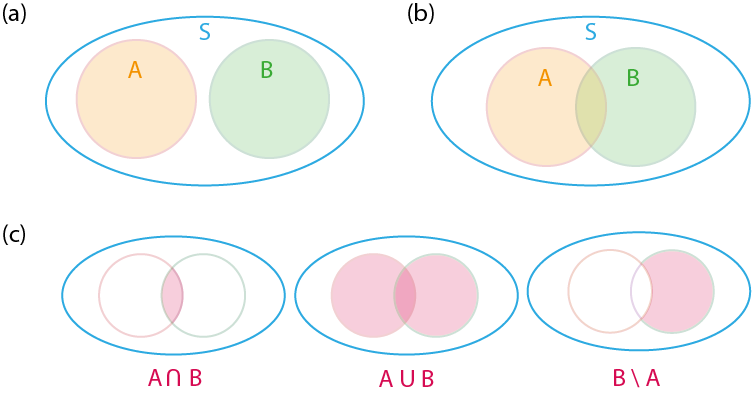
\includegraphics[width=0.6\textwidth]{Figures/venndiagramm.png}
\caption{Venn-Diagramme zur Veranschaulichung von Frequentistischen Wahrscheinlichkeiten. Die Ergebnisse $A$ und $B$ sind Teilmengen der Gesamtmenge $S$ aller möglichen Ergebnisse des Experiments. \textbf{(a)} Wenn die Ergebnisse $A$ und $B$ nicht gleichzeitig eintreten können, überlappen ihre Teilmengen im Venn-Diagramm nicht. \textbf{(b)} Wenn die Ergebnisse $A$ und $B$ gleichzeitig eintreten können, gibt es einen gewissen Überlapp zwischen ihren Teilmengen. \textbf{(b)} Venn-Diagramme sind hilfreich, um Schnittmengen, Vereinigungsmengen und Differenzmengen darzustellen.  }
\label{fig:venn}
\end{figure}

 Die Wahrscheinlichkeit $P(A \cup B)$, dass entweder Ereignis $A$ oder Ereignis $B$ eintritt, ist
\begin{align}
P(A \cup B) = P(A) + P(B) - P(A\cap B),
\label{eq:kombp}
\end{align}
wobei wir die Wahrscheinlichkeit $P(A\cap B)$ des gleichzeitigen Auftretens beider Ergebnisse subtrahieren müssen, um im Fall von überlappenden Ergebnismengen die entsprechende Fläche des Venn-Diagramms nicht doppelt zu zählen. Weiterhin ist häufig die  konditionelle  (auch: bedingte) Wahrscheinlichkeit $P(A|B)$, dass Ergebnis $A$ eintritt, wenn $B$ eintritt, von Interesse. Sie ist gegeben als
\begin{align}
P ( A | B ) = \frac{P ( A \cap B )}{P ( B )}.
\label{eq:kondp}
\end{align}
  Da $P(A \cap B) = P(B \cap A)$ können wir folgend aus Gleichung \ref{eq:kondp} den  Zusammenhang
\begin{align}
P ( A \cap B ) = P ( A | B ) P ( B ) = P ( B | A ) P ( A )\
\label{eq:bayespre}
\end{align}
 zwischen $P(A|B)$ und $P(B|A)$ herstellen. Aus diesem folgt schliesslich der sogennannte Satz von Bayes,
\begin{align}
P ( B | A ) = \frac{P ( A | B) P ( B )}{P ( A )}. 
\label{eq:bayes}
\end{align}

Die bisherige Betrachtung ist unabhängig davon, ob ein kausaler Zusammenhang zwischen $A$ und $B$ herrscht, korrekt. Falls kein solcher Zusammenhang besteht, d.h. $A$ und $B$ vollkommen unabhängig sind, entsprechen die bedingten Wahrscheinlichkeiten einfach den individuellen Wahrscheinlichkeiten der Ergebnisse, d.h.  
\begin{align}
P ( A | B ) = P(A). 
\end{align}
Weiterhin gilt dann
\begin{align}
 P ( A \cap B ) = P ( A ) P ( B ).
\end{align}

\subsection{Wahrscheinlichkeitsverteilungen - Grundlegende Charakteristiken}

Dem frequentistischen Wahrscheinlichkeitsbegriff folgend stellt das aus den Ergebnissen der wiederholten Messung der Zufallsvariablen erhaltene Histogramm (siehe Fig.~\ref{fig:messfehler1}) in einer diskreten Form die Wahrscheinlichkeiten als Funktion des Messwertes da. Es bildet somit, sofern zum Einen eine ausreichend hohe Anzahl an Wiederholungen durchgeführt wurde und zum Anderen sowohl die vertikale als auch horizontalen Auflösungen der Messung es zulassen, näherungsweise die zugrundeliegende (kontinuierliche) Wahrscheinlichkeitsverteilung der Messgrösse ab. Im Folgenden werden wir zunächst einige grundlegende Charakteristiken von Wahrscheinlichkeitsverteilungen definieren und dann auf einige relevante, konkrete Wahrscheinlichkeitsverteilungen eingehen. \\ 

Eine Wahrscheinlichkeitsverteilung ist eine positive und normierte Funktion, die die Verteilung der Wahrscheinlichkeit einer Zufallsvariablen $x$ beschreibt.  Falls die Zufallsvariable nur diskrete Werte annehmen kann, spricht man von einer sogenannten  \textbf{Probability Mass Function} (PMF), die jedem möglichen, diskreten Wert $x_n$ der Zufallsvariable eine Wahrscheinlichkeit $P(x_n)$ zuordnet. Es gilt 
\begin{align}
0 \leq P(x_n) \leq 1,
\end{align}
sowie
\begin{align}
\sum_n P(x_n) = 1.
\end{align}
Im Falle einer kontunierlichen Zufallsvariablen $x$ sprechen wir von einer  \textbf{Probability Density Function} (PDF) (zu deutsch: Wahrscheinlichkeitsdichtefunktion) $f(x)$ die
\begin{align}
0 \leq  f(x) 
\end{align}
und
\begin{align}
\int_{-\infty}^{\infty} f(x) = 1
\end{align}
erfüllt. Während im diskreten Fall die Wahrscheinlichkeit für das Auftreten eines bestimmten Wertes $x_n$ direkt aus der PMF abgelesen werden kann, entspricht im kontinuierlichen Fall $f(x)$ nicht direkt der Wahrscheinlichkeit für das Auftreten eines Wertes $x$. Stattdessen kann die Wahrscheinlichkeit dafür, dass das Ergebnis $x$ in in einem Intervall zwischen $a$ und $b$ liegt, durch Integration der PDF als  
\begin{align}
P(a\leq x \leq b) = \int_a^bf(x)dx
\end{align}
erhalten werden. \\

In Tabelle \ref{tab:pdfs} sind einige der wichtigsten Kennzahlen von Wahrscheinlichkeitsdichtefunktionen aufgelistet.

\begin{longtable}{p{3cm}|p{6cm}|p{5cm}}
\caption{Auflistung einiger wichtiger Kennzahlen von Wahrscheinlichkeitsdichtefunktionen.} \\
\textbf{Name und Variable} & \textbf{Formel} & \textbf{Bedeutung} \\ \hline \hline
Modus \gls{gl:xmode} & \begin{align}
\gls{gl:xmode}: \frac{d f ( x )}{dx}\bigg|_{\gls{gl:xmode}} = 0 
\end{align} & Der Wert von $x$, bei dem die Verteilung ihr Maximum erreicht. Die hier angegebene Formel zur Berechnung kann für eine PDF mit einem einzigen Maximum verwendet werden. \\ \hline 
Median $x_{\mathrm{median}}$ & \begin{align}
\frac{1}{2} = \int_{-\infty}^{x_{\mathrm{median}}} f ( x ) dx\
\end{align}  & Die Mitte der Verteilung. Der Median wird häufig bei der Darstellung von sozioökonomischen Daten verwendet, etwa zur Angabe des durchschnittlichen Gehalts einer Gesellschaft. \\ \hline
Halbwertsbreite  \gls{gl:FWHM} & \begin{align} \begin{split}
f ( a ) = f ( b ) = \frac{1}{2} f (\gls{gl:xmode} ) \\  \gls{gl:FWHM} = b - a\,.
\end{split} \end{align} & Charakterisiert die Breite der Verteilung beim halben Wert ihres Maximalwertes. \\ \hline
Erwartungswert \gls{gl:mu} & \begin{align} \begin{split} \mu = E(x) \\ = \int_{-\infty}^{+\infty} xf(x)dx \end{split} \end{align} & Die Zahl, die die Zufallsvariable $x$ im Mittel annimmt. Häufig wird der Erwartungswert auch als Mittelwert bezeichnet. \\ \hline
Varianz \gls{gl:var} &   \begin{align} \begin{split} \gls{gl:var} = E((x-\gls{gl:mu})^2) \\ = \int_{-\infty}^{+\infty} (x-\gls{gl:mu})^2f(x)dx \end{split} \end{align} &  Die mittlere quadratische Abweichung der Zufallsvariablen $x$ von ihrem Erwartungswert. \\ \hline
Standardabweichung \gls{gl:sigma} & \begin{align} \gls{gl:sigma} = \sqrt{\gls{gl:var}} \end{align} 
\label{tab:pdfs}
\end{longtable}

Zusätzlich zu diesen Charakteristika lassen sich für viele PDF sogenannte Momente berechnen. Das $m$-te Moment $M_m$ einer Wahrscheinlichkeitsverteilung $f(x)$ ist definiert als
\begin{align}
M_m = \int_{-\infty}^{+\infty} x^mf(x)dx.
\end{align}
Das 0-te Moment
\begin{align}
M_0 = \int_{-\infty}^{+\infty} f(x)dx = 1
\end{align}
entspricht somit der Normierungsbedingung der Wahrscheinlichkeitsverteilung, während das 1-te Moment
\begin{align}
M_1 = \int_{-\infty}^{+\infty} xf(x)dx = E(x)
\end{align}
ihren Mittelwert liefert. \\

Ebenfalls ist das $m$-te zentrale Moment einer Wahrscheinlichkeitsverteilung definiert als
\begin{align}
\Tilde{M}_m = \langle ( x - M_1 )^m \rangle\,.
\end{align}
Damit ist die Varianz einer PDF gegeben durch das zweite zentrale Moment:
\begin{align}
\sigma^2 = \langle ( x - M_1)^2 \rangle = \langle x^2 \rangle - \langle x \rangle^2 = M_2 - M_1^2\,.
\end{align}
Das dritte zentrale Moment quantifiziert die  Schiefe und das vierte zentrale Moment die Wölbung der PDF. Es ist hilfreich, die momenterzeugende Funktion zu definieren und unter Verwendung der Taylorreihe von $\exp ( \zeta x )$ zu formulieren
\begin{align}
\begin{split}
M ( \zeta ) = \int_{-\infty}^{+\infty} \exp ( \zeta x ) f ( x ) dx \\ 
= \int_{-\infty}^{+\infty} \left( 1 + \zeta x + \frac{ \zeta^2 x^2 }{ 2! } + \cdots \right) f ( x ) dx\\
= M_0 + \zeta M_1 + \frac{ \zeta^2 }{ 2! } M_2 + \cdots .
\end{split}
\end{align}
Höhere Momente $m \geq 1$ können iterativ aus der Ableitung der momenterzeugenden Funktion berechnet werden:
\begin{align}
M_m = \frac{ \partial^m M ( \zeta ) }{ \partial \zeta^m} \bigg|_{\zeta = 0}\,.
\end{align}\\

Darüber hinaus ist es hilfreich, die charakteristische Funktion $\phi(\nu)$
\begin{align}
\phi(\nu) = \int_{-\infty}^{+\infty} \exp ( \mathrm{i} \nu x) f ( x ) dx.
\label{eq:charakteristischefunktion}
\end{align}
 einer Wahrscheinlichkeitsverteilung $f(x)$ zu definieren, wobei $\mathrm{i}=\sqrt{-1}$ die imaginäre Einheit ist. Die charakteristische Funktion ist die inverse Fouriertransformierte der Wahrscheinlichkeitsverteilung. Die Fourier-Transformation werden wir in Kapitel \ref{ch:spectral} zur Spektralanalyse genauer kennenlernen.  Indem wir die Exponentialfunktion erweitern, können wir die charakteristische Funktion als Funktion der Momente der PDF ausdrücken:
\begin{align}
\begin{split}
\phi ( \nu ) & = \int_{-\infty}^{+\infty} \left( 1 + \mathrm{i} \nu x + \frac{ 1 }{ 2! } ( \mathrm{i} \nu )^2 x^2 + \frac{ 1 }{ 3! } ( \mathrm{i} \nu )^3 x^3 + \cdots \right) f ( x ) dx\\
& = 1 + \mathrm{i} \nu M_1 + \frac{ 1 }{ 2 ! } ( \mathrm{i} \nu )^2 M_2 + \frac{ 1 }{ 3! } ( \mathrm{i} \nu )^3 M_3 + \cdots\,.
\end{split}
\end{align}
Ausserdem können wir wir die Wahrscheinlichkeitsverteilung $f(x)$ durch Fouriertransformation von $\phi(\nu)$ berechnen:
\begin{align}
f ( x ) = \frac{ 1 }{ 2 \pi } \int_{-\infty}^{+\infty} \exp ( -\mathrm{i} \nu x ) \phi ( \nu ) d \nu\,.
\end{align}
Die Kombination dieser beiden Ergebnisse ergibt:
\begin{align}
f ( x ) = \frac{ 1 }{ 2 \pi } \int_{-\infty}^{+\infty} \exp ( -\mathrm{i} \nu x ) \left( 1 + \mathrm{i} \nu M_1 + \frac{ 1 }{ 2 ! } ( \mathrm{i} \nu )^2 M_2 + \frac{ 1 }{ 3! } ( \mathrm{i} \nu )^3 M_3 + \cdots \right)  d \nu\,.
\end{align}

\subsection{Die Normalverteilung}

In der Praxis finden wir sehr häufig normalverteilte Messergebnisse vor. Insbesondere liegt eine Normalverteilung immer dann vor, wenn der Messfehler  aus der additiven Überlagerung zahlreicher unabhängiger, zufälliger Ereignisse resultiert und somit selbst tatsächlich vollkommen zufällig ist.  Der Grund hierfür ist der sogenannte \textbf{zentrale Grenzwertsatz}:\\

\begin{center}
\begin{tcolorbox}[enhanced,width=6in,drop fuzzy shadow southwest,
    colframe=red!50!black,colback=red!05]
   Die Summe vieler (identisch verteilter)
Zufallsvariablen ist eine normalverteilte
Zufallsvariable. \\

\underline{Beispiel}: Während die Augenzahl beim Wurf eines einzelnen Würfels gleichverteilt ist, ist die Summe der Augenzahlen mehrerer Würfel normalverteilt.
\end{tcolorbox}
\end{center}

Die Normalverteilung wird daher häufig als Modell für die Wahrscheinlichkeitsverteilung von Messdaten angenommen, sofern keine Kenntnis über das Vorhandensein einer anderen, physikalisch motivierten Verteilung besteht. Sie wird durch den Erwartungswert \gls{gl:mu} und die Standardabweichung (die Quadratwurzel der Varianz) \gls{gl:sigma} $= \sqrt{ \gls{gl:var}}$ parametrisiert.
\begin{align}
f( x, \gls{gl:mu}, \gls{gl:sigma} ) = \frac{ 1 }{ \sigma \sqrt{ 2 \pi }} \exp{ \left( - \frac{ \left( x - \gls{gl:mu} \right)^2}{2 \sigma ^2} \right) }\,.
\label{eq:normalverteilung}
\end{align}
 Die Standardabweichung gibt hierbei das Gewicht der \gls{gl:PDF} um den Erwartungswert an: Ein Messergebnis liegt mit 68\,\% Wahrscheinlichkeit innerhalb des Intervalls $\left[ \gls{gl:mu} - \gls{gl:sigma} \text{, } \gls{gl:mu} + \gls{gl:sigma} \right]$. Je breiter das Intervall, desto mehr Gewicht, d.h. umso wahrscheinlicher ist es, ein Messergebnis im Intervall zu finden:
\begin{align}
\begin{split}
1\sigma & \rightarrow 68\,\% \\
2\sigma & \rightarrow 95\,\% \\ 
3\sigma & \rightarrow 99.7\,\% \\ 
& \cdots \\
5\sigma & \rightarrow 99.99994\,\%
\end{split}
\end{align}

Selbstverständlich sind die Parameter (\gls{gl:mu}, \gls{gl:sigma}) der Normalverteilung, die einer gemessenen Stichprobe zugrunde liegt, zunächst unbekannt und müssen anhand der experimentell gemessenen Daten möglichst gut abgeschätzt werden. Wir wollen dafür den Erwartungswert $E(x) =\gls{gl:mu}$ mit dem empirischen Mittelwert \gls{gl:xoverline}  und die Standardabweichung  \gls{gl:sigma} mit der empirischen Standardabweichung \gls{gl:deltax} annähern. Aber dürfen wir das?  \\ 

Um zu überprüfen, ob der empirische Mittelwert und die emprische Varianz gute Schätzwerte für den tatsächlichen Erwartungswert und die tatsächliche Varianz sind, bilden wir deren Erwartungswerte, $E(\Bar{x})$ und $E(\gls{gl:deltax2})$.  Zunächst berechnen wir den Erwartungswert des empirischen Mittelwertes:
\begin{align}
E(\Bar{x}) = E \left( \frac{1}{N} \sum_{n = 1}^N x_n \right) = \frac{1}{N} \sum_{n = 1}^N E(x_n)\,.
\end{align}
wobei wir verwendet haben, dass der Erwartungswert linear ist und somit für unabhängige Zufallsvariablen $X$, $Y$ sowie Konstanten $a$, $b$ gilt:
\begin{align}
\begin{split}
E(a) &= a\\
E(aX) &= a E(X)\\
E(aX + b) &= a E(X) + b\\
E(aX + bY) &= a E(X) + b E(Y)\,.
\end{split}
\end{align}
Wenn wir nun weiterhin beachten, dass jede einzelne Messung der Zufallsvariable den gleichen Erwartungswert besitzt wie die Zufallsvariable selbst (d.h. $E(x_n) = E(x)$) erhalten wir
\begin{align}
E(\Bar{x}) = \frac{1}{N} \sum_{n = 1}^N E(x_n)= \frac{1}{N} \sum_{n = 1}^N E(x) = \frac{1}{N} N E(x) = E(x)\,.
\end{align}
Der Erwartungswert des Mittelwertes entspricht also tatsächlich dem Erwartungswert der Zufallsvariablen. Der aus den Stichproben erhaltene empirische Mittelwert ist somit in der Tat ein guter Schätzwert für den tatsächlichen Erwartungswert:
\begin{align}
\mu \approx \overline{x} = \frac{1}{N} \sum^N_{n = 1} x_n\,,
\end{align}

Wir gehen nun analog vor für die Varianz und berechnen ihren Erwartungswert. Hierfür verwenden wir den Zusammenhang
\begin{align}
\text{var}(x) = E(x^2) - E(x)^2 \rightarrow E(x^2) = \text{var}(x) + E(x)^2
\end{align}
sowie
\begin{align}
\text{var}(\bar{x}) = \frac{\text{var}(x)}{N} 
\end{align}
und können damit folgende Umformung vornehmen: 
\begin{align}
\begin{split}
E(\gls{gl:deltax2}) &= E \left( \frac{1}{N-1} \sum_{n=1}^N ( \bar{x} - x_n )^2 \right)\\
&= E \left( \frac{1}{N-1} \sum_{n=1}^N ( \bar{x}^2 - 2 \bar{x} x_n + x_n^2 ) \right)\\
&= E \left( \frac{1}{N-1} \left( \sum_{n=1}^N \bar{x}^2 - 2 \sum_{n=1}^N \bar{x} x_n + \sum_{n=1}^N x_n^2 \right) \right)\\
&= E \left( \frac{1}{N-1} \left( N \bar{x}^2 - 2 \bar{x} \sum_{n=1}^N x_n + \sum_{n=1}^N x_n^2 \right) \right)\\
& = E \left( \frac{1}{N-1} \left( N \bar{x}^2 - 2 N \bar{x}^2 + \sum_{n=1}^N x_n^2 \right) \right)\\
&= E \biggl( \frac{1}{N-1} \biggl( \sum_{n=1}^N x_n^2 - N \bar{x}^2 \biggr) \biggr)\\
&= \frac{1}{N-1} \left( \sum_{n=1}^N E(x_n^2) - N E(\bar{x}^2) \right)\\
& = \frac{1}{N-1} \left( \sum_{n=1}^N (\text{var}(x) + E(x)^2 - N E(\bar{x}^2) \right)\\
& = \frac{1}{N-1} \left( \sum_{n=1}^N (\text{var}(x) + E(x)^2) - N \left( \frac{\text{var}(x)}{N} + E(\bar{x})^2 \right) \right)\\
&= \frac{1}{N-1} ( N \text{var}(x) - N E(x)^2 - \text{var}(x) + N E(\bar{x})^2 )\\
&= \frac{1}{N-1} (\text{var}(x) (N-1) - N E(x)^2 + N E(x)^2 ) \\
&= \frac{1}{N-1} \text{var}(x) (N-1) \\
&= \text{var}(x)\,.
\end{split}
\end{align}
Somit ist auch die empirische Standardabweichung ein guter Schätzwert der Standardabweichung.
\begin{align}
\gls{gl:sigma} \approx \gls{gl:deltax} = \sqrt{\frac{1}{N-1} \sum^N_{n = 1} \left( x_n - \gls{gl:xoverline} \right)^2}\,.
\end{align}

Jetzt, da wir die empirische Standardabweichung und Varianz als gute Schätzwerte für Erwartungswert und Varianz identifiziert haben, wollen wir zu unserem Datensatz an Messdaten für \gls{gl:g} aus Abschnitt \ref{chap:messfehler:sec:messfehler} zurückkehren. Zunächst wollen wir überprüfen, ob die von uns gemessenen Daten  tatsächlich einer Normalverteilung folgen. Wir berechnen, welcher Anteil unserer Messwerte im $1\sigma$-Intervall liegt und vergleichen das Resultat mit dem für die Normalverteilung erwarteten Wert.
\begin{lstlisting}[language = Python]
n_sigma = 0
width = 1
# Iteriere durch alle Bins und addiere ihre Werte auf, wenn sie im entsprechenden Intervall liegen
i = 0
for b in bins:
    if (b >= (mean - np.sqrt(var) * width)) and (b <= (mean + np.sqrt(var) * width)):
        n_sigma = n_sigma + occurrence[i]
    i = i + 1
print('Occurences within the {:d}-sigma-interval: {:0.1f}%'.format(width,n_sigma/N*100))
\end{lstlisting}
Wir finden, dass 64.7 Prozent unserer Messung im $1\sigma $ Intervall liegen, was sehr nah am erwarteteten Wert für die Gaussverteilug liegt. Auch entsprechende Berechnungen für die grösseren Intervalle liefern Ergebnisse, die sehr ähnlich zu den erwarteten Werten sind. Unsere Stichprobe scheint tatsächlich normalverteilt zu sein. \\ 

In einem weiteren Schritt simulieren wir nun unter der Annahme einer Normalverteilung und unter Verwendung unserer empirisch gemessenen Mittelwerts und Standardabweichung als Schätzungen der Parameter einen Datensatz mit höherer vertikaler Auflösung. Hierzu verwenden wir das random-Modul in Python:
\begin{lstlisting}[language = Python]
g_sim = np.random.normal(mean, np.sqrt(var), N)
\end{lstlisting}
Wir analysieren die so erhaltenen Werte analog zu unserem ursprünglichen Datensatz, verwenden nun allerdings deutlich schmälere Bins und normalisieren die erhaltenen Ereignishäufigkeiten nicht nur mit der Anzahl $N$ der Messungen, sondern ebenfalls mit der Bin-Breite, um eine Wahrscheinlichkeitsdichte (\textit{Probability Density})  zu erhalten.  Ebenfalls zeichnen wir die zugehörige Normalverteilung als Graph ein (siehe Figur \ref{fig:messfehler2}). Dieser Vergleich versinnbildlicht, dass eine Messung mit ausreichender Anzahl Datenpunkten und entsprechender Auflösung die zugrundeliegende Wahrscheinlichkeitsverteilung sehr gut abbilden kann.

\begin{figure}[H]
\centering
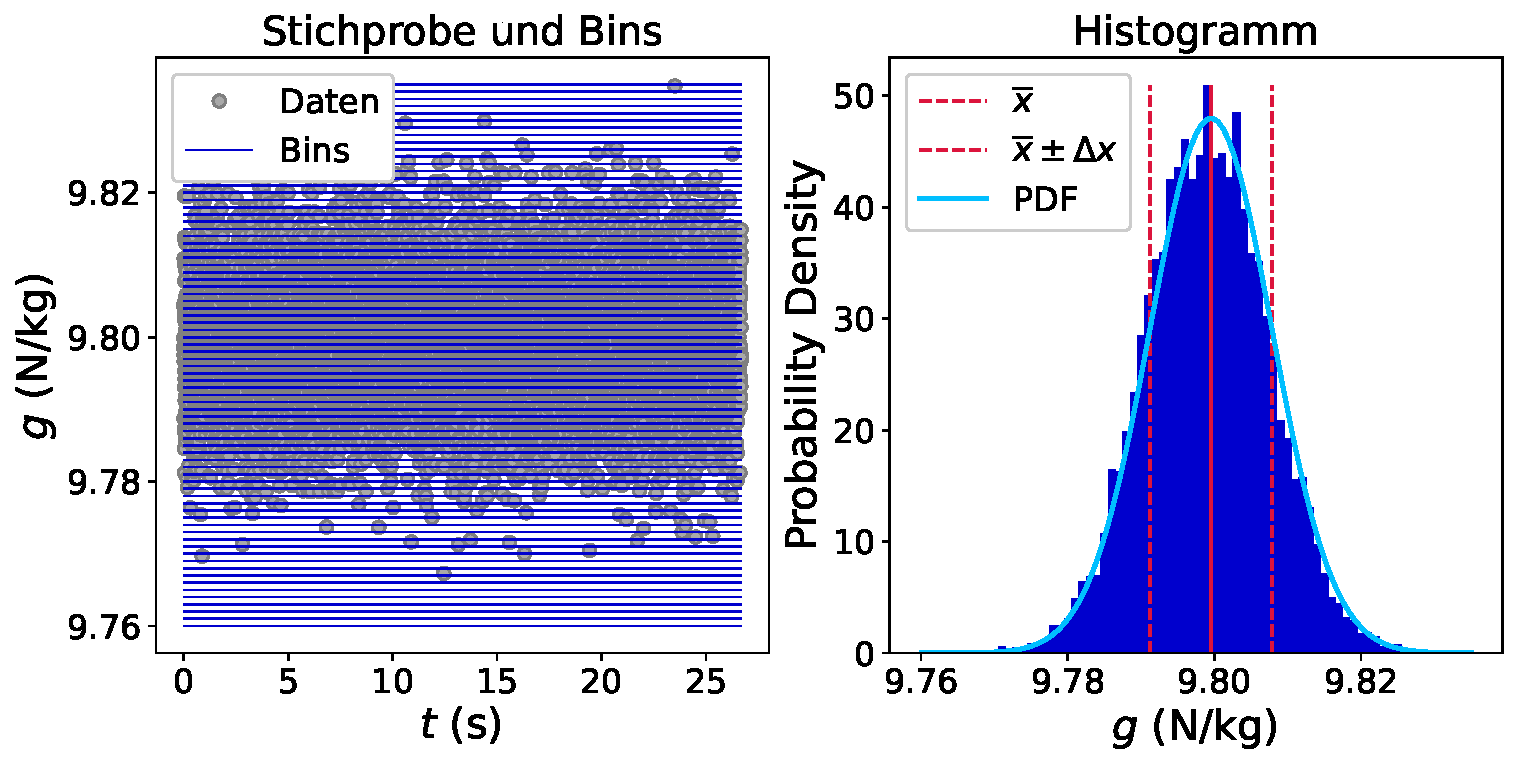
\includegraphics[width=0.9\textwidth]{Figures/messfehler2.pdf}
\caption{Statistische Analyse einer simulierten Messung von \gls{gl:g} mit höherer Auflösung. \textbf{Links:} Auftragung der gemessenen Datenpunkte (graue Punkte) gegen die Zeit $t$. Die Kanten der ``Bins'' sind als horizontale Linien indiziert.   \textbf{Rechts:} Das resultierende Histogramm der Stichprobe. Die Anzahl der Messergebniss pro Bins wurden für diese Darstellung bereits mit dem Produkt aus Anzahl der Datenpunkte $n$ und Bin-Breite normalisiert, um eine Wahrscheinlichkeitsdichte zu erhalten. Der empirische Mittelwert und die empirische Standardabweichung (rote Linien), sowie die aus diesen erhaltene Normalverteilung (blaue Linie) sind eingezeichnet.}
\label{fig:messfehler2}
\end{figure}


\subsection{Binomial- und Poissonverteilung}
Die Binomialverteilung ist eine der wichtigsten, diskreten Wahrscheinlichkeitsverteilungen. Sie liegt immer dann vor, wenn eine Serie von $n$ unabhängigen und gleichartigen Versuchen zur Messung einer Zufallsvariablen mit lediglich zwei möglichen Ergebnissen, $d$ und $u$, durchgeführt wird. Ein typisches Alltagsbeispiel für eine Binomialverteilung wäre etwa der Münzwurf, ein Beispiel der statistischen Physik die Besetzung eines Zustandes mit einer Reihe von Spins, die sich entweder in einem \glqq up\grqq{} (d.h. $S_z = +\frac{1}{2}\hbar$) oder \glqq down\grqq{} (d.h. $S_z = -\frac{1}{2}\hbar$) Zustand befinden können. Die Wahrscheinlichkeiten für die beiden Ergebnisse sind in jeder Durchführung des Versuchs identisch und  
\begin{align}
P(u) = p,
\end{align}
\begin{align}
P(d) = q = 1-p.
\end{align}
Die Binomialverteilung 
\begin{align}
B(k|p, n) = \frac{ n! }{ k! (n - k)! }p^k (1-p)^{n-k}
\end{align}
gibt die Wahrscheinlichkeit $B(k|p, n)$ dafür an, dass in $n$ Versuchen $k$-mal das Ergebnis $u$ auftritt. Sie setzt sich zusammen aus der der Wahrscheinlichkeit $p^k (1-p)^{n-k}$ für das Auftreten der $k$ Ereignisse in einer bestimmten Reihenfolge und dem Binomialkoeffizienten
\begin{align}
\begin{pmatrix} n\\ k \end{pmatrix} \equiv \frac{ n! }{ k! (n - k)! },
\end{align}
der angibt, auf wie viele verschiedene Arten man aus einer Menge von $n$ Objekten $k$ Objekte auswählen kann. Als Wahrscheinlichkeitsverteilung muss dies natürlich normiert sein, sodass wir als 0-tes Moment 
\begin{align}
M_0 = \sum_{k = 0}^n \begin{pmatrix} n\\ k \end{pmatrix} p^k q^{n-k} = 1
\end{align}
erhalten.  Wir wollen nun die höheren Momente ($m \geq 1$) mithilfe der Ableitung der Momenterzeugenden Funktion
\begin{align}
M_m = \frac{ \partial^m M (\zeta) }{ \partial \zeta^m} \bigg|_{\zeta = 0}
\end{align}
berechnen. Wir berechnen die Ableitung als
\begin{align}
\begin{split}
\frac{ \partial M_m }{ \partial p } &= \frac{ \partial }{ \partial p } \left( \sum_{k = 0}^n k^m \begin{pmatrix} n \\ k \end{pmatrix} p^k (1 - p)^{n-k} \right)\\
&= \sum_{k = 0}^n k^{m + 1} \begin{pmatrix} n \\ k \end{pmatrix} p^{k - 1} (1 - p)^{n - k} - \sum_{k = 0}^n k^m (n - k) \begin{pmatrix} n \\ k \end{pmatrix} p^k (1 - p)^{n - k - 1}\\
&= \frac{1}{p} \sum_{k = 0}^n k^{m + 1} \begin{pmatrix} n \\ k \end{pmatrix} p^k q^{n - k} - \frac{n}{q} \sum_{k = 0}^n k^m \begin{pmatrix} n \\ k \end{pmatrix} p^k q^{n - k} + \frac{1}{q} \sum_{k = 0}^n k^{m + 1} \begin{pmatrix} n \\ k \end{pmatrix} p^k q^{n - k}\\
&= \frac{1}{p} M_{m + 1} - \frac{n}{1} M_m + \frac{1}{q} M_{m + 1}.
\end{split}
\end{align}
und können somit die höheren Momente mittels 
\begin{align}
M_{m + 1} = n p M_m + p q \frac{ \partial M_m }{ \partial p } 
\end{align}
berechnen. Wir erhalten somit das erste Moment, den Mittelwert der Binomialverteilung, als 
\begin{align}
\mu = M_1 = n p M_0 + p q \frac{ \partial M_0 }{ \partial p } = np.
\end{align}
Für das zweite Moment folgt
\begin{align}
M_2 = n p M_1 + p q \frac{ \partial M_1 }{ \partial p } = np(np) + pq \frac{ \partial }{ \partial p } (np) = n^2 p^2 + npq ,
\end{align}
sodass wir für Standardabweichung und die Varianz schlussendlich folgende Ausdrücke erhalten:
\begin{align}
\sigma^2 = M_2 - M_1^2 = n p q \,,
\end{align}
\begin{align}
\sigma \propto \sqrt{n}.
\end{align}

Sofern ein Grenzfall vorliegt, in dem gilt
\begin{itemize}
    \setlength\itemsep{0em}
        \item Die Anzahl der Messungen $n$ ist sehr gross.
        \item Die Anzahl der Ereignisse pro Messung $k$ ist klein, insbesondere $n \gg k$.
        \item Die Wahrscheinlichkeit für ein Event $p$ ist sehr klein $(p \rightarrow 0)$.
\end{itemize}
geht die Binomialverteilung in die Poissonverteilung über. Die Poissonverteilung stellt somit einen Grenzfall der Binomialverteilung dar. Um die Poissonverteilung zu erhalten, müssen wir die Binomialverteilung wiefolgt umformen
\begin{align}
\lim_{n \gg k} \begin{pmatrix} n \\ k \end{pmatrix} p^k (1 - p)^{n - k} = \lim_{n \gg k} \frac{ n! }{ k! (n - k)! } p^k (1 - p)^{n - k} = \frac{ n^k }{ k! } p^k (1 - p)^n
\end{align}
und erhalten schliesslich durch Einsetzen des Mittelwertes $\mu = np$  und Bilden des Grenzwertes $\lim_{p \rightarrow 0} (1 - p)^{\frac{1}{p}} = e^{-1}$  die Poisson-Verteilung 
\begin{align}
P_{\mu}(k) = \frac{ \mu^k }{ k! } \exp(-\mu) . 
\end{align}
Analog zur Binomialverteilung können wir nun ausgehend von $M_0 = 1$ iterativ mittels
\begin{align}
 M_{m + 1} = \mu M_m + \mu \frac{ \partial M_m }{ \partial \mu }
\end{align}
die höheren Momente der Poissonverteilung berechnen. Wir erhalten somit für den Mittelwert der Poissonverteilung
\begin{align}
 M_1 = \mu M_0 + \mu \frac{ \partial M_0 }{ \partial \mu } = \mu.
\end{align}
Für die Varianz erhalten wir:
\begin{align}
M_2 = \mu M_1 + \mu \frac{ \partial M_1 }{ \partial \mu } = \mu^2 + \mu\,,\\
\sigma^2 =  M_2 - M_1^2 = \mu\,.
\end{align}

\subsection{$\chi^2$ Verteilung}
Die $\chi^2$ Verteilung ist eine Verteilung, die insbesondere bei der Analyse der Güte von Fits verwendung findet. 

Wir betrachten zunächst zwei unkorrelierte, normalverteilte Zufallsvariablen $\epsilon_1$ und $\epsilon_2$ mit ihren Erwartungswerten $\mu_1 = \mu_2 = 0$ und Varianzen $\sigma_1$ und $\sigma_2$.
Dann ist die Wahrscheinlichkeit, Werte in den Intervallen $\left[ \epsilon_1, \epsilon_1 + d\epsilon_1 \right]$ und $\left[ \epsilon_2, \epsilon_2 + d\epsilon_2 \right]$ zu finden, gegeben durch:
\begin{align}
f(\epsilon_1, \epsilon_2)d\epsilon_1 d\epsilon_2 = \frac{1}{\sqrt{2 \pi} \sigma_1} \exp{ \left( - \frac{ \epsilon_1^2}{2 \sigma_1^2} \right)} \frac{1}{\sqrt{2 \pi} \sigma_2} \exp{ \left( - \frac{ \epsilon_2^2}{2 \sigma_2^2} \right)}d\epsilon_1 d\epsilon_2.
\label{eq:vl2-3}
\end{align}

Wir definieren neue Variablen $x_1 = \frac{\epsilon_1}{\sigma_1}$ und $x_2 = \frac{\epsilon_2}{\sigma_2}$, damit wird \ref{eq:vl2-3} zu:

\begin{align}
f(\epsilon_1, \epsilon_2)dx_1 dx_2 = \frac{1}{2 \pi} \exp{ \left( - \frac{1}{2} \left( x_1^2 + x_2^2\right) \right)} dx_1 dx_2.
\end{align}

Weiterhin definieren wir die Summe der Quadrate: $S = x_1^2 + x_2^2$.

Die Wahrscheinlichkeit, dass $S$ in einem Intervall $\left[ S, S + dS \right]$ liegt, entspricht also der Fläche eines Rings um den Ursprung mit Radius $\chi$ und Breite $d\chi$. Um dies zu berechnen, wechseln wir in Polarkoordinaten:

\begin{align}
x_1 = \chi \cos{(\theta)}\\
x_2 = \chi \sin{(\theta)}\\
\chi^2 = S = x_1^2 + x_2^2\\
\end{align}

Damit finden wir:

\begin{align}
f(\epsilon_1, \epsilon_2)dx_1 dx_2 = f(\chi, \theta) \chi d\chi d\theta = \frac{1}{2 \pi} \exp{ \left( - \frac{1}{2} \chi^2 \right)} \chi d\chi d\theta,
\end{align}

und nach Integration über $\theta$:

\begin{align}
f(\chi) \chi d\chi = \exp{ \left( - \frac{1}{2} \chi^2 \right)} \chi d\chi.
\end{align}

Dies können wir ausdrücken als Funktion von $\chi^2$:

\begin{align}
f(\chi^2) d\chi^2 = \frac{1}{2}\exp{ \left( - \frac{1}{2} \chi^2 \right)} d\chi^2,
\end{align}

und ohne die Differentiale finden wir die PDF der Zufallsvariable $\chi^2$:

\begin{align}
f_2(\chi^2) = \frac{1}{2}\exp{ \left( - \frac{1}{2} \chi^2 \right)}.
\end{align}

Dies ist die $\chi^2$ Verteilung für zwei Variablen, also für zwei Freiheitsgrade. Verallgemeinert für $k$ Freiheitsgrade (bzw. $k$ unabhängige, normalverteilte Zufallsvariablen) ergibt sich:

\begin{align}
f_k(\chi^2) = \frac{(\chi^2)^\frac{k-2}{2}}{s^\frac{k}{2} \left( \frac{k}{2}-1 \right)!} \exp{ \left( - \frac{1}{2} \chi^2 \right)}.
\end{align}

Diese Funktion ist mühsam zu berechnen. Man findet ihre Werte in Tabellen oder in Python in der Bibilothek SciPy:
\begin{lstlisting}[language = Python]
from scipy.stats import chi2
\end{lstlisting}
Um $f_n(\chi^2)$ zu berechnen, kann dann die folgende Funktion verwendet werden:
\begin{lstlisting}[language = Python]
f_X2_k = chi2.pdf(X2, k)
\end{lstlisting}

Wir listen hier einige Eigenschaften der $\chi^2$ Verteilung auf, ohne diese herzuleiten. Die Mode der $\chi^2$ Verteilung, also ihr Maximum, wird erreicht für: 
\begin{align}
\chi^2_\mathrm{mode} = k-2.
\end{align}
Der Erwartungswert der Verteilung ist:
\begin{align}
E(\chi^2) = k,
\end{align}
und ihre Varianz ist
\begin{align}
\mathrm{var}(\chi^2) = 2k.
\end{align}

Oft ist es praktisch, die reduzierte $\chi^2$-Verteilung zu verwenden: $\chi^2_\mathrm{red}=\frac{1}{k}\chi^2$. Dies hat den Vorteil, dass $E(\chi^2_\mathrm{red}) = 1$ ist, unabhängig von $k$. Dies gilt jedoch nicht für ihre Varianz: $\mathrm{var}(\chi^2_\mathrm{red}) = \frac{2}{k}$.


\section{Fehler des Mittelwertes und die Integrationszeit}

Nachdem wir nun nun den frequentistischen Wahrscheinlichkeitsbegriff eingeführt und damit unsere erste intuitive Interpretation des Histogramms als Annäherung der Wahrscheinlichkeitsverteilung unserer Messgrösse fundiert haben, wollen wir uns einem weiteren Aspekt des Histogramms in   Fig.~\ref{fig:messfehler1} zuwenden. Bei näherer Betrachtung ziehen wir folgende Vermutung: Während die Unsicherheit einer einzelnen Messung durch die Standardabweichung \gls{gl:deltax} gegeben ist, können wir aus einer grossen Anzahl Datenpunkten den Mittelwert viel genauer abschätzen. Im Histogramm sehen wir beispielsweise bereits sehr deutlich, in welchen Bin der Erwartungswert sein sollte. Die Standardabweichung scheint also die Präzision unserer Messung des Mittelwerts nicht fundamental zu begrenzen, wenn wir bereit sind, genug Zeit für viele Messungen aufzubringen.

%Ein wichtiger Parameter in unseren vorangegangenen Analysen ist die Anzahl der Wiederholungen $n$, die in einem echten Experiment proportional zur Messzeit und somit limitiert ist.  Da sich die der Messung zugrundeliegende  PDF nicht mit $n$ ändert, bleiben die  \\ 

Um diese Vermutung mathematisch beweisen, berechnen wir den zufälligen Fehler $\Delta{\mu}$, den wir bei der Abschätzung des Erwartungswertes $\mu$ aus dem Mittelwert $\overline{x}$ einer begrenzten Anzahl von Messwerten machen. Wir bezeichnen diesen Schätzfehler als ``Fehler des Mittelwertes'' (engl: Error of the Mean). Wir führen also eine Messung mit $N$ Werten durch und berechnen daraus einen Mittelwert. Diese Messreihe wiederholen wir nun viele Male und bilden die Varianz der einzelnen Mittelwerte. Daraus können wir erschliessen, wie unterschiedlich die verschiedenen Mittelwerte voneinander sind. Für diese Varianz gilt:
\begin{align}
\Delta{\mu}^2 = \text{var} \left( \overline{x} \right) = \text{var} \left( \frac{1}{N} \sum^N_{n=1} x_n \right) = \frac{1}{N^2} \text{var} \left( \sum^N_{n=1} x_n \right) = \frac{1}{N^2} N \sigma^2 = \frac{1}{N} \sigma^2\,.
\label{eq:vl3-1}
\end{align}
Die Wurzel der Varianz zeigt uns die Unsicherheit des Mittelwerts, und somit den Fehler, den wir bei der Abschätzung des Erwartungswertes aus dem Mittelwert von $N$ Messungen machen.  Dieser Fehler ist somit $\Delta \mu = \frac{ \sigma }{ \sqrt{N} }$. Wir können durch wiederholtes Messen also die Genauigkeit des Messergebnisses verbessern. Generell halten wir fest: Die Werte von \gls{gl:mu} und  \gls{gl:sigma} ändern sich nicht systematisch durch wiederholtes Messen. Die zugehörigen Schätzfehler, die wir bei der Annäherung dieser Werte mit den empirischen Werten machen, ändern sich allerdings sehr wohl. Im Limit unendlich vieler Messungen ($N  \rightarrow  \infty)$ entsprechen empirischer Mittelwert und empirische Standardabweichungen den tatsächlichen Parametern der zugrundeliegenden Verteilungen, solange keine systematischen Fehler vorliegen.

\section{Fehlerfortpflanzung}
\label{chap:fehler:sec:fehlerfortpflanzung}

Wir haben nun gelernt, wie wir den Fehler (die Unsicherheit) der Messung einer Variablen charakterisieren können. Häufig können wir allerdings die Grösse, an der wir interessiert sind, nicht direkt messen. Stattdessen messen wir experimentell zugängliche Parameter und berechnen aus diesen die eigentliche Zielgrösse. Zum Beispiel kann die Erdbeschleunigung, die wir im vorangegangenen Beispiel betrachtet haben, auch experimentell mit einem Fadenpendel bestimmt werden
\begin{align}
g = \frac{4 \pi^2 l}{T_{Periode}^2}\,.
\label{eq:vl2-2}
\end{align}
Hierbei werden die die Fadenl\"ange \gls{gl:l} und Periodendauer \gls{gl:T_Periode} experimentell gemessen und die Erdbeschleunigung entsprechend berechnet.  Um zu verstehen, wie sich die Fehler der Messungen von \gls{gl:l}  und \gls{gl:T_Periode} auf den Fehler der Bestimmung von \gls{gl:g} auswirken, müssen wir eine sogenannte Fehlerfortpflanzung durchführen. Die Fehlerfortpflanzung ermöglicht es uns, den Einfluss von Fehlern in den einzelnen gemessenen Variablen auf den Fehler des berechneten Resultates zu bestimmen. Die exakte Formel hierfür kann grundsätzlich sehr komplex sein. Im Folgenden wollen wir eine Methode zur Fehlerfortpflanzung näher betrachten, die es uns ermöglicht, den Fehler zumindest im Fall von normalverteilten PDF auf eine einfache Weise anzunähern. 


\subsection{Fehlerfortplfanzung nach Gauss}

Wir betrachten zunächst den einfachsten Fall, in dem unsere Zielgrösse $f (x)$ nur von einer einzigen, fehlerbehafteten Messgrösse $x$ abhängt. Um zu analysieren, wie sich eine Unsicherheit $\Delta x$ in $x$ auf die Unsicherheit  $\Delta f(x) $ von $f (x)$ auswirkt, bilden wir die  Taylorentwicklung von $f(x)$ am Ort $\overline{x}$ und brechen diese nach dem ersten Glied ab (lineare Näherung, Taylorentwicklung erster Ordnung):
\begin{align}
f(x)  = f ( \overline{x} + \Delta x ) \approx f ( \overline{x} ) + \frac{\partial f}{\partial x}\bigg|_{\overline{x}} \left( x - \overline{x} \right) = f ( \overline{x} ) + \frac{\partial f}{\partial x}\bigg|_{\overline{x}} \Delta x.
\end{align}
Wir erhalten somit den folgenden Zusammenhang zwischen dem Fehler der Zielgrösse, $\Delta f(x) $, der aus der Abweichung  $\Delta x$ entsteht:
\begin{align}
\Delta f(x) =  f ( \overline{x} + \Delta x ) - f ( \overline{x} )  =  \frac{\partial f}{\partial x}\bigg|_{\overline{x}} \Delta x.
\end{align}
Unter der Annahme, dass die Messung von $x$ einer Normalverteilung folgt, können wir die Standardabweichung $\sigma_x$ als  typischen Fehler $\Delta x$ einsetzen und wollen auch $\Delta f(x)$ als Standardabweichung $\sigma_f$ interpretieren.  
\begin{align}
\sigma_f =   \frac{\partial f}{\partial x}\bigg|_{\overline{x}} \sigma_x.
\end{align}
Folglich erhalten wir für den Zusammenhang der Varianzen
\begin{align}
\sigma_f^2 = \left( \frac{\partial f}{\partial x}\bigg|_{\overline{x}} \right)^2\sigma_x^2.
\end{align}

\begin{figure}[H]
\centering
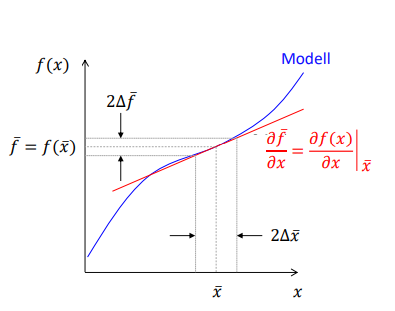
\includegraphics[width=0.5\textwidth]{Figures/gauss1D.png}
\caption{Veranschaulichung des Prinzips der Gausschen Fehlerfortplanzung im eindimensionalen Fall.}
\end{figure}

Wir betrachten nun den etwas komplizierteren Fall, in dem unsere Zielgrösse $f(x,y)$ von zwei fehlerbehafteten Messgrössen $x, y$ abhängt.Analog zum eindimensionalen Fall versuchen wir, einen Zusammenhang zwischen der Varianz der Zielgrösse und den Varianzen der Messgrössen $\sigma_x, \sigma_y$ herzustellen. Hierbei verwenden wir die Taylorentwicklung erster Ordnung für beide Variablen. Der Übersichtlichkeit halber verwenden wir $\overline{f} = f(\overline{x}, \overline{y})$, $f_n = f(x_n, y_n)$ und $\frac{\partial f}{\partial x}\bigg|_{\overline{x}, \overline{y}} = \frac{\partial \overline{f}}{\partial x}$:
\begin{align}
\begin{split}
\sigma_f^2 = \frac{1}{N-1} \sum_{n=1}^N (f_n - \overline{f})^2 = \frac{1}{N-1}\sum_{n=1}^N \left( \frac{\partial \overline{f}}{\partial x} (x - \overline{x}) + \frac{\partial \overline{f}}{\partial y} (y - \overline{y})\right)^2  \\
=  \frac{1}{N-1}\sum_{n=1}^N \left[ \left(\frac{\partial \overline{f}}{\partial x}\right)^2 (x - \overline{x})^2 + \left(\frac{\partial \overline{f}}{\partial y}\right)^2 (y - \overline{y})^2 + 2\frac{\partial \overline{f}}{\partial x}\frac{\partial \overline{f}}{\partial y}(x - \overline{x})(y - \overline{y})\right] \\
= \left(\frac{\partial \overline{f}}{\partial x}\right)^2\sigma_x^2 +  \left(\frac{\partial \overline{f}}{\partial y}\right)^2\sigma_y^2 + 2\frac{\partial \overline{f}}{\partial x}\frac{\partial \overline{f}}{\partial y}\sigma_{xy}^2
\end{split}
\label{eq:Gauss2D}
\end{align}
Wie aus Gleichung \ref{eq:Gauss2D} ersichtlich wird, hängt der Fehler der Zielgrösse im mehrdimensionalen Fall zusätzlich zu den Varianzen der einzelnen Messgrössen ($\sigma_x\sigma_y$) auch noch von der sogenannten Kovarianz $\sigma_{xy}^2$ ab, die wir im folgenden Kapitel \ref{chap:korrelation:sec:kovarianz} noch genauer betrachten wollen. Den in Gleichung \ref{eq:Gauss2D} erhaltenen Ausdruck können wir auch unter Verwendung der sogenannten Kovarianzmatrix schreiben als:
\begin{align}
\sigma_f^2 = (\partial_x, \partial_y)f \begin{pmatrix}
\sigma_x^2 & \sigma_{xy}^2 \\
\sigma_{xy}^2 & \sigma_y^2 
\end{pmatrix} \begin{pmatrix}
\partial_x \\
\partial_y 
\end{pmatrix} f
\end{align}
Dieser Formalismus kann auf beliebig viele Variablen erweitert werden, mit entsprechend höherer Dimensionalität der Kovarianzmatrix. Für unkorrelierte Variablen (d.h. alle Kovarianzen sind null, die Kovarianzmatrix ist diagonal) erhalten wir mit diesem Verfahren der Fehlerfortpflanzung:
\begin{align}
\sigma^2_f &= \sum^N_{n=1} \left( \frac{\partial f}{\partial x_n} \right)^2 \sigma^2_{x_n}\,,
\label{eq:GaussnD}
\end{align}
\begin{align}
\sigma_f &= \sqrt{ \sum^N_{n=1} \left( \frac{\partial f}{\partial x_n} \right)^2 \sigma^2_{x_n}}\,.
\label{eq:vl3-4}
\end{align}
Folglich gilt für unkorrelierte Variablen, dass die Varianz der Summe gleich der Summe der Varianzen ist.\\

Dies ist die sogenannte \textbf{Gauss-Methode} der Fehlerrechnung. Sie setzt voraus, dass:
\begin{itemize}
    \setlength\itemsep{0em}
        \item die $\sigma_n$ klein genug sind, um eine lineare Taylor-Approximation annehmen zu dürfen.
        \item die $x_n$ statistisch unabhängig sind, so dass gilt: $\text{var} ( x_1 + x_2 ) = \text{var} ( x_1 ) + \text{var} ( x_2 )$. Falls die $x_n$ nicht statistisch unabhängig sind, nennen wir sie korreliert und es treten zusätzliche Kovarianzen auf (siehe Kapitel \ref{chap:korrelation}) 
\end{itemize}

Wir wollen die Gaussche Fehlerfortpflanzung nun für unser Beispiel der Bestimmung der Erdbeschleunigung mittels der Messung der Schwingungsperiode  und Länge eines Fadenpendels verwenden. Wir messen die Schwingungsperiode \gls{gl:T_Periode}  zu:
\begin{align*}
\gls{gl:T_Periode} = \bigl( \underarrow[\text{2.50}][\uparrow]{\text{$\overline{T}$}} \pm \underarrow[\text{0.08}][\uparrow]{\text{$\sigma_T$}} \bigr) \text{s}
\end{align*}
und die Fadenlänge \gls{gl:l}  zu:
\begin{align*}
\gls{gl:l} = \bigl( \underarrow[\text{1.55}][\uparrow]{\text{$\overline{l}$}} \pm \underarrow[\text{0.02}][\uparrow]{\text{$\sigma_l$}} \bigr) \text{m}\,.
\end{align*}

Mit der Fehlerfortpflanzung nach Gauss ergeben sich folgende partielle Ableitungen:
\begin{align}
\frac{\partial \gls{gl:g}}{\partial \gls{gl:T_Periode}} = - \frac{8 \pi^2 \gls{gl:l}}{\gls{gl:T_Periode}^3},
\end{align}
\begin{align}
\frac{\partial \gls{gl:g}}{\partial \gls{gl:l}}  =   \frac{4 \pi^2}{\gls{gl:T_Periode}^2}.
\label{eq:vl3-7}
\end{align}
Damit folgt letztendlich:
\begin{align}
\sigma_g = \sqrt{ \left(  - \frac{8 \pi^2 \gls{gl:l}}{\gls{gl:T_Periode}^3} \right)^2 \sigma^2_T + \left(\frac{4 \pi^2}{\gls{gl:T_Periode}^2} \right)^2 \sigma^2_l }\,,
\label{eq:vl3-8}
\end{align}
wobei wir $\overline{T}$ und $\overline{l}$ einsetzen.



\subsection{Signifikante Stellen}
Aus den vorangegangenen Diskussionen dieses Kapitels haben Sie bereits gelernt, dass keine experimentell gemessene Zahl absolut genau ist. Dieser Umstand sollte sich auch in der Anzahl Stellen widerspiegeln, mit denen ein numerisches Resultat angegeben wird. Es ist wichtig, Resultate mit der richtigen Anzahl Stellen anzugeben, denn zu viele angegebene Stellen suggerieren eine falsche Genauigkeit. Die Anzahl Stellen vor und hinter dem Komma, die man mit Sicherheit angeben kann, wird als \textit{Anzahl signifikanter Stellen} bezeichnet. \\

%Als Daumenregel gilt: Ein Resultat sollte nicht mehr signifikante Stellen haben als der ungenaueste Wert, der zur Berechnung verwendet wurde.
Wir runden Zahlen auf die letzte Ziffer, die vom berechneten Messfehler betroffen ist. Der Messfehler wiederum wird üblicherweise auf eine signifikante Stelle gerundet. Zum Beispiel würden wir das Ergebnis der Messung einer Masse mit Mittelwert $m = 3.25118$ kg mit Standardabweichung $\sigma_m =0.02$ kg angeben als $m=3.25\text{ kg}\pm 0.02  
 \text{ kg}$. Wir haben folgende Optionen, um Standardfehler (Fehler des Mittelwerts) anzugeben:
 \begin{enumerate}
     \item[-] Absoluter Fehler $x + \Delta x$, z.B. Die Masse beträgt $m=3.25\text{ kg}\pm 0.02$ kg  
     \item[-] Relativer Fehler  $x + \frac{\Delta x}{x}$, z.B. Die Masse beträgt $m=3.25\text{ kg}\pm 1\%$ 
     \item[-] Implizite Angabe, z.B. Die Masse beträgt $m=3.25\text{ kg}$. Hier wird angenommen, dass die Zahl nicht genauer bekannt ist als die Hälfte der letzten angegebenen Ziffer (d.h. hier $\pm 0.005$).
 \end{enumerate}
%\subsection{Mit Monte-Carlo Simulationen }
%Es sei wieder die Funktion $f ( x_1, x_2, x_3, ..., x_n )$ im nachfolgenden unser Modell mit dem Beispiel der Amplitude eines Resonators: $A = f ( S, g, V_\text{in}, f, ... )$.\\[0.3cm]
%Als Monte Carlo Simulation bezeichnen wir ein ``numerisches Experiment'', in dem wir einen Wert viele Male mit zuf\"allig verteilten Anfangswerten berechnen. Die Anfangswerte können einer beliebigen PDF folgen.
%\begin{itemize}
%    \setlength\itemsep{0em}
%        \item[$-$] Keine analytische L\"osung.
%       \item[$-$] MC Simulation kann sehr rechenintensiv sein.
%        \item[$+$] Beliebig nichtlineare und komplexe Fehler berechenbar.
%        \item[$+$] Nicht auf normalverteilte \gls{gl:PDF}s beschr\"ankt.
%\end{itemize}


\newpage


\begin{tcolorbox}[enhanced,width=6in,
    fontupper=\small,drop fuzzy shadow southwest,
    colframe=black!50!black,colback=black!5]
\textbf{Verständnisfragen:} \\
\begin{enumerate}
\item[1] Wodurch entstehen Abweichungen zwischen dem
gemessenen Mittelwert und dem «Literaturwert»?
\item[2] Wodurch entsteht eine Standardabweichung in der
gemessenen Verteilung von Messwerten?
\item[3] Wie verändert sich nach wiederholtem Messen der Fehler in der
Abschätzung des Erwartungswertes ($\Delta\mu$) und die Standardabweichung ($\sigma$)?
\item[4] Kann der Fehler in der Abschätzung des Erwartungswertes $\Delta\mu$ kleiner werden als die Standardabweichung $\sigma$?
\end{enumerate}
\end{tcolorbox}

\begin{tcolorbox}[enhanced,width=6in,
    fontupper=\small,drop fuzzy shadow southwest,
    colframe=black!50!black,colback=black!5]
\textbf{Antworten:} \\
\begin{enumerate}
\item[1] Für unendlich viele Messpunkte tragen nur
systematische Fehler zu dieser Abweichung bei. Für
endlich viele Messpunkte werden auch statistische
Fehler wichtig.
\item[2] Die Standardabweichung ist ein gängiges Mass für die
statistische Streuung von Messwerten.
\item[3] $\sigma$ bleibt unverändert, aber $\Delta \mu $ wird kleiner. 
\item[4] Ja.
\end{enumerate}
\end{tcolorbox}